\chapter{DeepTAM\authorB}

\section{What is DeepTAM?}
DeepTAM provides a keyframe-based dense camera tracking and depth map estimation system that is entirely learned. The idea of DeepTAM is based on DTAM \cite{dtam}.The generic idea is: drift-free camera tracking via a dense depth map towards a keyframe and aggregation of depth over time. But the way to implement this concept is different. In the DeepTAM deep networks are used for tracking and mapping.These networks learn only from data. It also processes more than two images for the 6 DOF egomotion and depth estimation. With that it can avoid the drift of the use of keyframes and as more keyframes come in it can refine the depth map.

\section{Tracking}
The main objective is to estimate a 4 x 4 transformation matrix T. This matrix maps a point in the keyframe coordinate system to the coordinate system of the current camera frame.
\newline
DeepTAM uses an more efficient way. It generates a virtual keyframe and tries to predict the increment instead of trying to estimate T. For more details see \cite{ZUB19a}. 

\subsection{Network Architecture}

\begin{figure}[h]
	\centering
	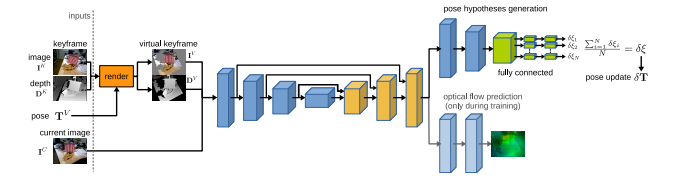
\includegraphics[width=1.1\textwidth]{./media/images/DeepTAM_schematic.PNG}
  	\caption{Schematic of DeepTAM
  	\\Source: \url{http://lmb.informatik.uni-freiburg.de/Publications/2019/ZUB19a}}
  	\label{DeepTAMschematic}
\end{figure}

To estimate the 6 DOF pose between a keyframe and an image the encoder-decoder-based architecture is used. To estimate camera motion you have to relate the keyframe to the current image. Because of that DeepTAM uses optical flow as an supportive task. With this optical flow the network is ensured to take advantage of the relationship between both frames. It uses two network branches for predicting the pose. One is the optical flow prediction and the other is the pose hypotheses generation. This improves the accuracy for the pose prediction.

\section{Mapping}

DeepTAM computes a set of depth maps every keyframe. For good quality depth maps, information will be accumulated in a cost volume. From this cost volume the depth map will be extracted by means of a convolutional neural network.

\subsection{Network Architecture}

\subsection{Training}
In about 8 days in total the training of the mapping network can be acomplished on a NVIDIA GTX 1080Ti.

\gls{optical-flow}



